\documentclass[11pt,a4paper]{article}

\usepackage[latin1]{inputenc} 
\usepackage[spanish]{babel}
\decimalpoint
\setlength{\parskip}{0.5\baselineskip} 
\usepackage{fullpage}
\usepackage[procnames]{listings}
\usepackage{fancyhdr}
\usepackage{lastpage}
\usepackage{xcolor}
\usepackage{booktabs}
\usepackage{graphicx}
\usepackage{subcaption}
\usepackage[fleqn]{amsmath}
\parindent 0in 
\setlength{\mathindent}{0pt}
\usepackage{float}
\usepackage{hyperref}

% \hypersetup{
%   pdfkeywords={DEV,unity,Light-bot,LuisCostero,UCM,MII},
%   pdfsubject={{DEV Proyecto final de la asignatura. Luis Costero}},
%   pdfcreator={pdflatex - Luis Costero}}


%% DEFINICIONES
\newcommand{\TODO}[1]{{\huge \color{red} \textbf{TODO: }#1 }}
\newcommand{\todo}[1]{{\large \color{red} \textbf{TODO: }#1 }}
\newcommand{\HRule}{\rule{\linewidth}{0.5mm}}



\definecolor{bluekeywords}{rgb}{0,0,1}
\definecolor{greencomments}{rgb}{0,0.5,0}
\definecolor{redstrings}{rgb}{0.64,0.08,0.08}
\definecolor{xmlcomments}{rgb}{0.5,0.5,0.5}
\definecolor{types}{rgb}{0.17,0.57,0.68}

\lstset{language=[Sharp]C,
  captionpos=b,
  numbers=left, %Nummerierung
  numberstyle=\tiny, % kleine Zeilennummern
  frame=lines, % Oberhalb und unterhalb des Listings ist eine Linie
  showspaces=false,
  showtabs=false,
  breaklines=true,
  showstringspaces=false,
  breakatwhitespace=true,
  escapeinside={(*@}{@*)},
  commentstyle=\color{greencomments},
  morekeywords={partial, var, value, get, set},
  keywordstyle=\color{bluekeywords},
  stringstyle=\color{redstrings},
  basicstyle=\ttfamily\small,
}

%%%%%%%%%%%%%%%%%%%%%%%%%%%%%%%%%%%%%%%%%%%%%%%%%%%%%%%%%%%%%%%%%%%%%%%%%%%%%%%%
\begin{document} 

\begin{titlepage}

  \begin{center}


    % Upper part of the page
    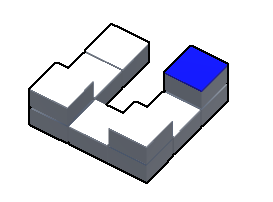
\includegraphics[width=0.4\textwidth]{./images/title.png}\\[1cm]    

    \textsc{\LARGE Universidad Complutense de Madrid}\\[1.5cm]

    \textsc{\Large Desarrollo de videojuegos}\\[0.5cm]


    % Title
    \HRule \\[0.4cm]
           { \huge \bfseries Light Bot}\\[0.4cm]
           
           \HRule \\[1.5cm]

           \begin{center}
             \Large
             \textbf{URL:} \url{https://youtu.be/zPJi_PGFbf8}
           \end{center}
           \vspace{2cm}
           % Author and supervisor
           \hfill\emph{Autor:}\\
           \hfill Luis Mar�a Costero Valero
           
           \vfill
           
           % Bottom of the page
           {\large Febrero 2016}
           
  \end{center}
  
\end{titlepage}

\tableofcontents


\newpage{}
\part{El juego}
\section{El juego}
\subsection{Introducci�n}
\label{s1:subsec:introduccion}
Con el objetivo de introducir a ni�os en edades tempranas en el mundo
de la inform�tica, en los �ltimos a�os se han realizado grandes
esfuerzos en la creaci�n de herramientas sencillas que sirvan como una
primera introducci�n a la programaci�n.

El ejemplo m�s conocido es Scratch\cite{scratch}, consistente en un
lenguaje de programaci�n visual que permite, mediante interacciones
\emph{drag\&drop} y un sistema de encaje de fichas de puzzle,
construir programas funcionales sin mucha dificultad.\\

Alternativamente a la creaci�n de lenguajes de programaci�n orientados
a este fin, existen multitud de juegos con este prop�sito, donde la
idea com�n a todos ellos es la de guiar a un personaje en un tablero
para alcanzar diferentes objetivos. Para que el personaje se mueva, el
usuario tendr� que programar la secuencia de movimientos que este ha
de realizar. Algunos de estos juegos pueden ser
Cargo-Bot\cite{cargo-bot}, Bee-bot\cite{bee-bot} o
Light-bot\cite{light-bot}.


\subsection{Descripci�n del juego}
\label{s1:subsec:descripcion}
El videojuego creado se basa en el juego \emph{light
  bot}\cite{light-bot}. El objetivo del juego es mover al personaje
principal (representado por un cilindro y un cubo) por el tablero con
el objetivo de colorear todas las casillas marcadas en azul en un
color amarillo. Para ello, el usuario posee una serie de botones en la
parte derecha de la pantalla con los que puede ordenar al robot
realizar distintas �rdenes que luego ejecutar� en la parte
izquierda. La imagen~\ref{s1:fig:interfaz} muestra une ejemplo de la
interfaz.

\begin{figure}[h]
  \begin{minipage}{0.5\textwidth}
    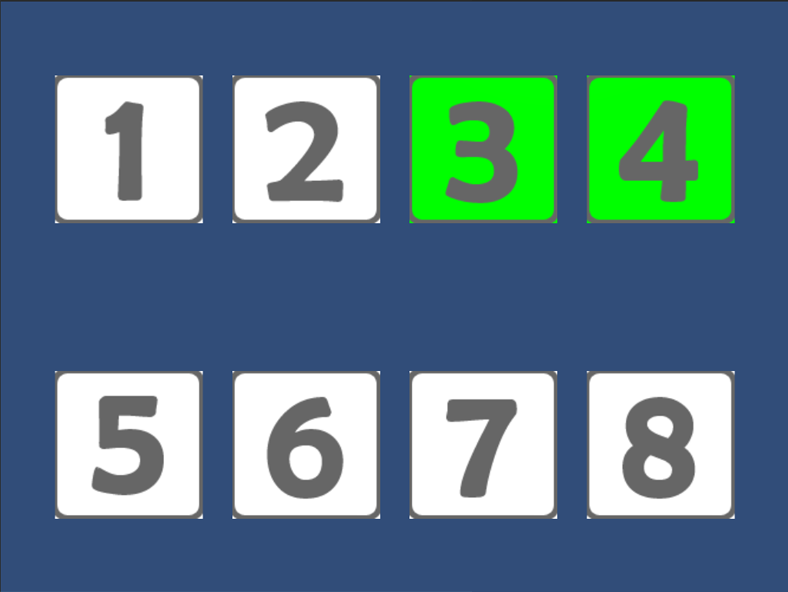
\includegraphics[width=\textwidth]{images/interfaz_menu.png}
  \end{minipage}
  \begin{minipage}{0.5\textwidth}
    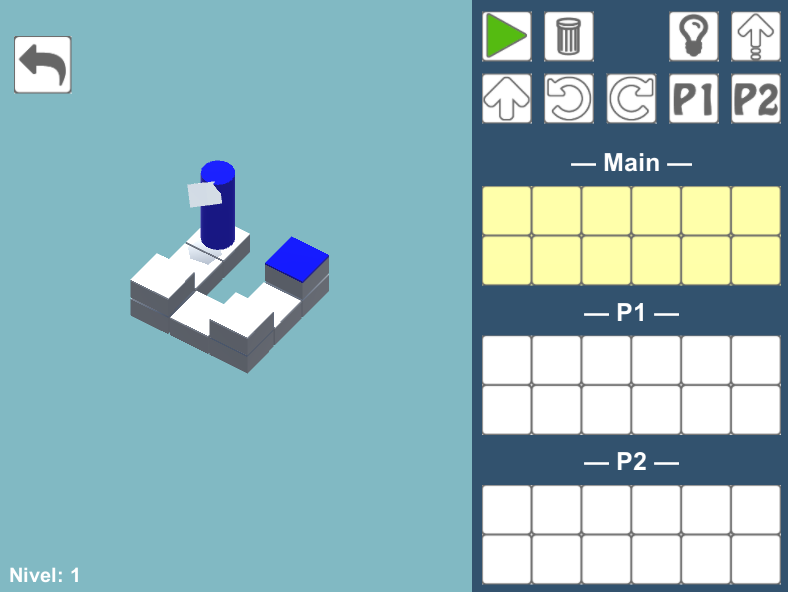
\includegraphics[width=\textwidth]{images/interfaz.png}
  \end{minipage}
  \caption{Ejemplo de la interfaz del juego}
  \label{s1:fig:interfaz}
\end{figure}


Como se puede observar en al figura, la pantalla del juego se
encuentra dividida en dos zonas (derecha e izquierda). La zona
izquierda muestra al robot y el tablero, y una vez introducidos los
comandos, es donde estos se reproducir�n. La parte derecha de la
pantalla la forman los distintos comandos que puede ejecutar el
personaje, y permite al jugador combinarlos para superar el nivel.

La forma que tiene el jugador de interactuar con el juego es haciendo
clicks en los distintos comandos que se presentan, coloc�ndolos en los
paneles que aparecen para posteriormente ejecutarlos. Los comandos
que puede realizar el usuario son:

\begin{table}[h]
  \centering
  \begin{tabular}{|c|c|c|c|c|c|c|}\hline
    
\includegraphics[scale=0.5]{./images/actions/up.png} &
    
\includegraphics[scale=0.5]{./images/actions/right.png} &
    
\includegraphics[scale=0.5]{./images/actions/left.png} &
    
\includegraphics[scale=0.5]{./images/actions/jump.png} &
    
\includegraphics[scale=0.5]{./images/actions/light.png} &
    
\includegraphics[scale=0.5]{./images/actions/p1.png} &
    
\includegraphics[scale=0.5]{./images/actions/p2.png} \\ \hline \hline
    Avanzar & Girar dcha. & Girar izq. & Saltar & Iluminar & Proc. 1 &
    Proc. 2 \\\hline
  \end{tabular}
\end{table}

Debajo de los comandos aparecen los tres paneles en los que el jugador
puede insertar los comandos (\emph{Main}, \emph{P1} y \emph{P2}
respectivamente). Cuando se reproduzcan los comandos seleccionados, el
robot comenzar� a reproducir los comandos que se encuentran en el
panel \emph{Main}, y si encuentra alg�n comando \emph{P1} o \emph{P2},
pasar� a reproducir los comandos de estos paneles. Destacar que las
llamadas a \emph{P1} y \emph{P2}, no tienen por qu� realizarse siempre
desde \emph{Main}, permitiendo as� anidamiento de llamadas a funci�n,
o incluso bucles en forma de llamadas recursivas sin condici�n de
fin\footnote{Aunque una llamada recursiva sin condici�n de fin pueda
  parecer un bucle infinito, el juego detecta la condici�n de victoria
cuando todas las casillas marcadas en azul se encuentran de color
amarillo, por lo que la condici�n de fin viene impl�citamente dada por
que el n�mero de casillas azules sea 0.}.

Al hacer click en una orden, esta se anota en el panel activo que est�
en ese momento. El panel activo se identifica porque tiene el fondo de
un color distinto (en la figura~\ref{s1:fig:interfaz} el panel activo
es el panel \emph{Main}, que tiene el fondo de color amarillo). Para
seleccionar que panel se encuentra activo es suficiente con hacer
click encima de �l.

Adicionalmente a estos elementos, el jugador posee tres botones m�s
con los que interactuar:
\begin{itemize}
  \item \emph{Play:} Al pulsar este bot�n, el robot comienza a
    reproducir los movimientos de los paneles. El usuario ya no puede
    modificar las �rdenes hasta que el robot finalice. El color de los
    paneles cambia y el bot�n de play se transforma en un bot�n de
    stop.
  \item \emph{Borrar:} Situado a la derecha del bot�n \emph{play},
    permite eliminar las �rdenes del usuario cuando el robot se
    encuentra parado.
  \item \emph{Volver al men�:} Situado en la esquina superior
    izquierda, permite regresar al men� de selecci�n de niveles en
    cualquier momento de la partida.
\end{itemize}



Al hacer click en los distintos paneles, se selecciona el panel activo
en el que insertar las �rdenes. Cuando un panel est� activo, se indica
cambiando en color del fondo del panel (en la
figura~\ref{s1:fig:interfaz} se ve como el fondo del panel \emph{Main}
se encuentra de un color amarillo).\\

\textbf{Reproducci�n}\\

Una vez que el usuario ha introducido los comandos que desea que el
robot realice y haya pulsado el bot�n de play, el juego pasa a la fase
de reproducci�n de los comandos. En esta fase, el usuario ya no puede
pulsar ning�n bot�n salvo el de parar la reproducci�n, y el robot ir�
ejecutando las �rdenes una a una, mientras se refleja en la parte
izquierda de la pantalla.

\begin{figure}
  \centering
  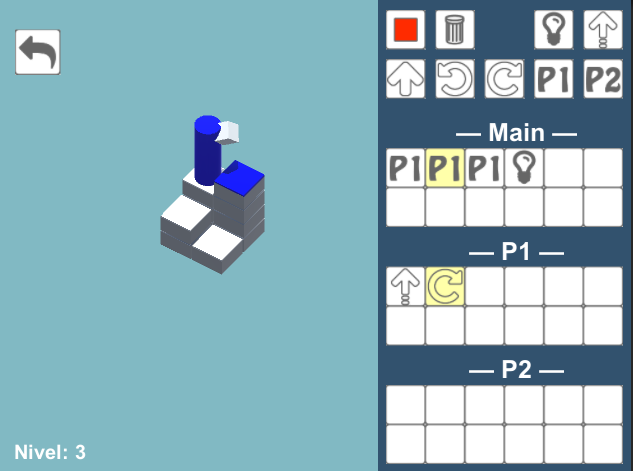
\includegraphics[width=0.65\textwidth]{./images/interfaz_play.png}
  \caption{El robot reproduciendo las �rdenes introducidas.}
  \label{s1:fig:interfaz_play}
\end{figure}


En la figura~\ref{s1:fig:interfaz_play} se puede observar como el
robot est� ejecutando los comandos introducidos para superar el nivel
3. Como se observa, el bot�n de \emph{play} se ha sustituido por el
bot�n de \emph{stop}, que volver� a colocar al robot en su posici�n
original y permitir� al usuario seguir introduciendo comandos.

Adicionalmente a estos cambios, el comando que est� ejecutando el
robot en el momento se iluminar�, permitiendo asociar cada comando con
un movimiento. En la figura se observa como el robot est� ejecutando
la segunda llamada a la funci�n \emph{P1}, dentro de la cual est�
realizando el movimiento de giro hacia la derecha.

Cuando un nivel es superado, se informa al usuario de esto mediante un
cartel en la pantalla, y se vuelve a cargar la pantalla de selecci�n
de nivel, pero indicando en color verde qu� niveles ya han sido
superados y cuales no.


\subsection{Caracter�sticas principales}
\label{s1:subsec:caracteristicas_principales}
Aunque el juego se ha descrito en las secciones anteriores, aqu� se
presenta un resumen de las principales caracter�sticas del juego
relacionadas con la jugabilidad y las din�micas del juego. En el
pr�ximo cap�tulo se detallar�n los aspectos relativos a la
implementaci�n.

\begin{itemize}
  \item Pantalla de selecci�n de men�. A trav�s de esta pantalla el
    jugador puede seleccionar qu� nivel desea superar. Tambi�n sirve
    de control para ver que niveles se han superado con anterioridad o
    no. El jugador puede volver a esta pantalla en cualquier momento
    del juego.
  \item M�ltiples paneles donde introducir los comandos. Al existir
    distintos paneles, existe la idea de panel activo, que el jugador
    puede cambiar en cualquier momento mientras se encuentra
    introduciendo comandos.
  \item Llamadas entre paneles. El usuario puede introducir llamadas
    entre paneles mediante los comandos \emph{P1} y \emph{P2}. De esta
    manera se permite simular llamadas a funci�n, llamadas a funci�n
    anidadas, y llamadas recursivas.
  \item Modo ejecuci�n. Cuando el robot se encuentra reproduciendo los
    comandos el usuario no puede insertar o borrar los comandos
    introducidos, siendo necesario parar la ejecuci�n primero.
  \item Modo resaltado durante la ejecuci�n. Al ejecutar los distintos
    comandos, estos se iluminan permitiendo seguir la ejecuci�n de los
    mismos de manera visual.
\end{itemize}


%
%
%%%
%%% Local Variables:
%%% mode: latex
%%% TeX-master: "./main.tex"
%%% End:



\newpage{}

\part{Implementaci�n}
\section{Las c�maras del juego}
\label{s2:sec:camaras}
Como se ha descrito en la secci�n anterior, la interfaz del juego se
encuentra dividida en dos secciones claramente diferenciadas (derecha e
izquierda). Cada secci�n posee sus propios scripts para el dibujado de la
interfaz y el control de las acciones del usuario. Para relacionar ambas
partes, se utiliza un script de nombre \texttt{Director.cs} que se encarga
de comunicarse y coordinar ambas partes.

Para realizar esta divisi�n de la interfaz, se ha decidido utilizar dos
c�maras sobre regiones distintas del espacio, y configurarlas seg�n se
muestra en la figura~\ref{s2:fig:camaras} para que compartan la pantalla.

\begin{figure}[h]
  \begin{minipage}{0.5\textwidth}
    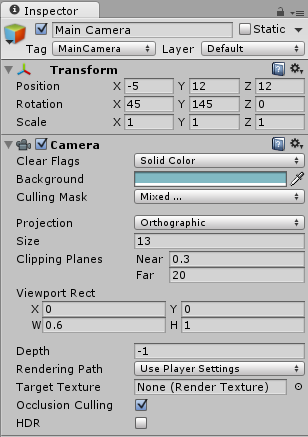
\includegraphics[width=\textwidth]{images/camaras/izq.png}
  \end{minipage}
  \begin{minipage}{0.5\textwidth}
    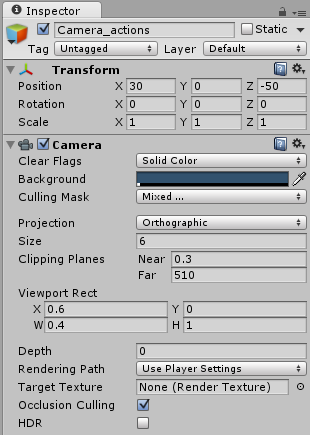
\includegraphics[width=\textwidth]{images/camaras/dcha.png}
  \end{minipage}
  \caption{Configuraci�n de las c�maras}
  \label{s2:fig:camaras}
\end{figure}

Adem�s, para evitar que los textos se rendericen en ambas c�maras, se han
creado dos capas nuevas y configurado el \emph{Culling Mask} de cada c�mara
para que cada una renderice una capa del juego.

\newpage{}

\section{El tablero del juego}
\label{s3:sec:tablero}

\subsection{Ficheros xml}
\label{s3:subsec:xml}
Para la implementaci�n de los niveles se ha decidido crear una estructura
xml que permita guardar cada nivel en un fichero independiente. De esta
manera, solamente es necesaria una escena que carga un mapa u otro
dependiendo del nivel elegido.

La estructura del fichero xml elegida consta de 3 partes bien
diferenciadas:
\begin{enumerate}
  \item \texttt{dimensions}: Representa el tama�o que va a tener cada celda
    del juego, las cubiertas, el tama�o del mapa y la escala respecto al
    prefab guardado.
  \item \texttt{board}: Representa a las casillas del tablero. Permite
    establecer una altura por defecto a cada celda. Adem�s, cada celda
    viene definida por las coordenadas (x,z), la altura y, y un atributo
    indicando si es una celda objetivo o no (\emph{goal}).
  \item \texttt{robot}: Indica la posici�n original del robot, y la
    rotaci�n con la que tiene que comenzar.
\end{enumerate}

En el c�digo~\ref{s3:lst:xml} se muestra un ejemplo de nivel, que
corresponde al nivel 1 mostrado en la figura~\ref{s1:fig:interfaz}.\\

\begin{lstlisting}[caption={Ejemplo de nivel 1 del juego}, label=s3:lst:xml]
<xml>
	<dimensions>
		<board length_x="10" length_z="10" scale="2"/>
		<block size="1" separation="0.1" />
		<cover size="0.1" />
		<robot height="2" />
	</dimensions>

	<board default_height="0" >	
		<tile x="2" z="0" height="1" />
		<tile x="2" z="1" height="1" />
		<tile x="2" z="2" height="2" />
		<tile x="1" z="2" height="1" />
		<tile x="0" z="2" height="2" />
		<tile x="0" z="1" height="1" />
		<tile x="0" z="0" height="2" attr="goal"/>	
	</board>
	
	<robot>
		<position x="2" y="1" z="0" />
		<rotation x="0" y="-90" z="0" />
	</robot>
</xml>
\end{lstlisting}

\subsection{Leyendo el fichero, creando el tablero}
Para la lectura del nivel en formato xml, y la creaci�n del tablero por
pantalla, se utiliza el script de nombre \texttt{GUI\_Layout.cs}, que
realiza ambas cosas. Para la creaci�n por pantalla, se utilizan prefabs que
representan a los bloques y cubiertas de los bloques, as� como los
distintos materiales usados para encender y apagas las celdas. Estos
elementos se asocian al script mediante la interfaz de unity.

Para almacenar las casillas internamente, se ha decidido almacenar de
manera separada la definici�n de la representaci�n visual. Para la
definici�n de la celda, se utilizan las siguientes estructuras, que m�s
tarde se utilizar�n desde el script:

\begin{minipage}{0.5\textwidth}
  \begin{lstlisting}
/* Definicion de una casilla. */
public class TileDef {
  public TileType type;
  private int _height;
  public int height {
    get{ return _height; }
    set{
      _height = value;
      if (value <= 0)
      type = TileType.none;
    }
  }
  
  public bool isOn;
  public int x;
  public int z;
}
  \end{lstlisting}
\end{minipage}
\begin{minipage}{0.5\textwidth}
  \begin{lstlisting}
/* Tipos para una casilla */
public enum TileType{
  normal,
  goal,
  none
}
  \end{lstlisting}
\end{minipage}


El script lo que realiza en primer lugar es la lectura del tablero xml
sobre las variables. Una vez le�do el tablero entero, se dibuja la interfaz
a partir de estas variables, y en �ltimo lugar se coloca al robot en su
posici�n correcta.

El m�todo que lee el fichero xml es el siguiente:
\begin{lstlisting}[caption={M�todo encargado de la lectura del fichero
      xml}]
/** Script encargado de toda la interfaz de la parte izquierda.
 * Crea el tablero a partir de un fichero xml, y coloca al robot en la posicion adecuada.
 * Almacena el tablero de forma logica para poder comprobar si los movimientos son posibles.
 * La representacion fisica de la representacion logica se encuentran almacenadas de manera independiente.
 */
public class GUI_Layout : MonoBehaviour {
  public static GUI_Layout S;//Singleton para acceder
  
  // Prfebs para crear una casilla
  public GameObject tileBlock_prefab;
  public GameObject specialCover_prefab;
  public GameObject normalCover_prefab;
  
  // Materiales para el cover de una casilla
  public Material offCover_material;
  public Material onCover_material;
  
  //Prefab del robot
  public GameObject robot_prefab;
  
  
  // Lectura del xml
  public PT_XMLReader      xmlr;  // PT_XMLReader
  public PT_XMLHashtable   xml;
  
  
  // Lista de xml para cada nivel
  public TextAsset[] niveles;
  
  
  // tamanyo maximo del tablero
  public int MAX_SIZE=20;
  
  //Texto para mostrar el numero de nivel
  public GameObject LevelTxt;
  
  
  public bool _____________________ ;
  public TextAsset texto;
  
  // Datos para pintar el mapa. Leidos del xml
  private float blockSize = 1f; 
  private float blockSeparation = 0.1f;
  private float coverSize = 0.1f; 
  private float scale = 2f;
  
  //Datos para pintar el robot. Leidos del xml
  private Vector3 robotPosition;
  private Vector3 robotRotation;
  private float robotHeight;
  
  //tamanyo del tablero
  private int size_x;
  private int size_z;
  private int default_height;
  
  // Definiciones e instancias de las celdas
  public TileDef[,] board_def;
  public GameObject[,] board;
  
  //Anchor para el board
  public GameObject boardAnchor;
  
  //Gameobject del robot para poder destruirlo
  public GameObject robot;
  
  
  
  public void Awake(){
    S = this;
    this.texto = this.niveles[levelLoad.level-1];
    
    GUIText gt = this.LevelTxt.GetComponent<GUIText>();
    gt.text = "Nivel: " + levelLoad.level;
  }
  
  
  public void Start(){
    this.resetLayout ();
    
    this.readLayout (texto.text);
    
    this.drawlayout ();
    this.drawRobot();
    
  }
  
  
  // -------------------------------------
  // -------------- METODOS --------------
  // -------------------------------------
  
  /*
   * carga el tablero definido en el xml pasado por paramtero
   */
  public void readLayout(string xmlText){
    //Antes de hacer nada, reseteamos el tablero
    this.resetLayout ();
    
    xmlr = new PT_XMLReader();
    xmlr.Parse(xmlText); 
    xml = xmlr.xml["xml"][0];
    
  
    //1.- Definiciones de las dimensiones
    PT_XMLHashtable dimensions = xml["dimensions"][0];
    //1.1 - tablero
    this.size_x = int.Parse (dimensions ["board"][0].att ("length_x"));
    this.size_z = int.Parse (dimensions ["board"][0].att ("length_z"));
    this.scale = float.Parse (dimensions ["board"][0].att ("scale"));
    
    //1.2 - bloque
    this.blockSize = float.Parse (dimensions ["block"][0].att ("size"));
    this.blockSeparation = float.Parse (dimensions ["block"][0].att ("separation"));
    
    //1.3 - cover
    this.coverSize = float.Parse (dimensions ["cover"][0].att ("size"));
    
    //1.4 - robot
    this.robotHeight = float.Parse (dimensions ["robot"][0].att("height"));
    
    
    //2.- Celdas por defecto
    this.default_height = int.Parse (xml ["board"] [0].att ("default_height"));
    this.initBoard (this.default_height, this.size_x, this.size_z);
    
    
    //3.- Definimos de las celdas
    PT_XMLHashList tileX = xml["board"][0]["tile"];
    for (int i=0; i<tileX.Count; i++) {
      int x, z;
      x = int.Parse (tileX[i].att("x"));
      z = int.Parse (tileX[i].att("z"));
      
      
      this.board_def[x, z].height = int.Parse(tileX[i].att ("height"));
      
      string attr = (tileX[i].HasAtt("attr")) ? tileX[i].att ("attr") : "none";
      switch (attr){
        case "goal":
          this.board_def[x,z].type=TileType.goal;
          Director.S.totalGoals ++;
          break;
        default:
          this.board_def[x,z].type = TileType.normal;
          break;
      }
      this.board_def[x,z].isOn = false;
    }
    
    //4.- Posicion inicial del robot.
    PT_XMLHashtable robot = xml["robot"][0]["position"][0];
    this.robotPosition = new Vector3(float.Parse(robot.att("x")),
                float.Parse(robot.att("y")),
                float.Parse(robot.att("z")));
    robot = xml["robot"][0]["rotation"][0];
    this.robotRotation = new Vector3(float.Parse(robot.att("x")),
                float.Parse(robot.att("y")),
                float.Parse(robot.att("z")));
    
    //Transformamos la rotacion en el intervalo [0,360)
    while(this.robotRotation.y < 0){
      this.robotRotation.y += 360;
    }
    while(this.robotRotation.y >=360){
      this.robotRotation.y -= 360;
    }
}
\end{lstlisting}


Una vez le�do los datos del tablero, se dibuja la interfaz asociada a este
tablero, y tambi�n se coloca el robot en su posici�n. Los m�todos
encargados de esto son los siguientes:

\begin{lstlisting}[caption={M�todos para dibujar el tablero y al robot}]
/** Dibuja los bloques del tablero segun la definicion guardada en this.board_def.
* Agrupa todos los elementos en un layout. Se supone que se ha invocado
* con anterioridad a resetLayout() que borra todos los hijos del anchor
* (es decir, borra todos los bloque creados)
*/
private void drawlayout(){
  GameObject tile;
  for (int i=0; i<this.size_x; i++) {
    for (int j=0; j<this.size_z; j++) {
      if(this.board_def[i,j].type == TileType.none)
      continue;
      
      //Creamos el tile
      tile = createTile(this.board_def[i,j].height, this.board_def[i,j].type == TileType.goal);
      tile.name = "" + i + "x" + j;
      //posicion segun la i, j
      tile.transform.position = new Vector3(i*(2*this.blockSize + this.blockSeparation), 0,
      j*(2*this.blockSize + this.blockSeparation));
      //hijo del anchor
      tile.transform.parent = this.boardAnchor.transform;
      
      //lo guardamos en el mapa
      this.board[i,j] = tile;
    }
  }
}

/** 
* Dibuja al robot en la posicion original leida del xml.
* El robot viene definido por una posicion inicial, y una direccion
* a la que se encuentra mirando.
*/
private void drawRobot(){
  GameObject robot = Instantiate(this.robot_prefab) as GameObject;
  
  //Colocar en la posicion y la rotacion
  robot.transform.position = new Vector3(this.robotPosition.x*(2*this.blockSize + this.blockSeparation),
  (this.robotPosition.y-1)*(this.blockSize + this.blockSeparation) + 
  this.robotHeight + this.blockSize/2 + this.coverSize,
  this.robotPosition.z*(2*this.blockSize + this.blockSeparation));
  
  robot.transform.rotation = Quaternion.Euler(this.robotRotation);
  
  //Calculamos la direccion a la que mira
  Vector3 dir;
  if(this.robotRotation.y < 90)
    dir = new Vector3(1,0,0);
  else if (this.robotRotation.y < 180)
    dir = new Vector3(0,0,-1);
  else if (this.robotRotation.y < 270)
    dir = new Vector3(-1,0,0);
  else 
    dir = new Vector3(0,0,1);
  
    ((Movement)robot.GetComponent<Movement>()).dirAct = dir;
    ((Movement)robot.GetComponent<Movement>()).rotAct = this.robotRotation;
    
    
    ((Robot)robot.GetComponent<Robot> ()).init ((int)(this.robotPosition.x), (int)(this.robotPosition.y), 
    (int)(this.robotPosition.z),
    (int)dir.x, (int)dir.z);
    
    this.robot = robot;
}


/*
* Resetea las variables necesarias para iniciar una nueva ejecucion.
*/
private void resetLayout(){
  this.board_def = new TileDef[MAX_SIZE, MAX_SIZE];
  if(this.board != null){
    for (int i=0; i<MAX_SIZE; i++)
    for (int j=0; j<MAX_SIZE; j++)
    Destroy(this.board[i,j]);
  }
  
  this.board = new GameObject[MAX_SIZE, MAX_SIZE];
  
  //Destruimos y volvemos a crear el boardAnchor
  if (this.boardAnchor != null) {
    Destroy (this.boardAnchor);
  }
  this.boardAnchor = new GameObject ();
  this.boardAnchor.name = "BoardAnchor";
  
  if(this.robot != null)
  Destroy(robot);
  
  Director.S.totalGoals = 0;
}


/*
 * Inicia el tablero de tamanyo nxm con celdas de altura h.
 * Si es una casilla fuera de n,m lo inicializa con una celda a none.
 */
private void initBoard (int h, int n, int m){
  TileDef td;
  for (int i=0; i<this.MAX_SIZE; i++) {
    for (int j=0; j<this.MAX_SIZE; j++) {
      td = new TileDef();
      td.x = i;
      td.z = j;
      td.height = h;
      
      
      if(i> n || j> m){ //fuera del tablero
	td.type = TileType.none;
	this.board_def[i,j] = td;
      } else { //Celda buena por defecto
	td.type = (h<=0) ? TileType.none : TileType.normal;
	this.board_def[i,j] = td;
      }
    }
  }
}

	
/*
 * Devuelve un objeto con una torre de bloques creada, de altura pasada por parametro.
 * El atributo special indica si es una casilla objetivo o no
 */
private GameObject createTile(int height, bool special){
  GameObject tile = new GameObject ();
  
  //1.- Bloques: escala, hijos del tile, apilar encima.
  GameObject go;
  for (int i = 0; i<height; i++){
    go = Instantiate(this.tileBlock_prefab) as GameObject;
    go.transform.localScale = new Vector3(this.scale, this.blockSize, this.scale);
    go.transform.parent = tile.transform; //hijo del tile
    go.transform.position = new Vector3(0, i*(this.blockSize + this.blockSeparation), 0); //encima del anterior
    go.name = "block_" + i;
  }
  
  //2.- Cover
  go = special ? Instantiate (this.specialCover_prefab) : Instantiate (this.normalCover_prefab);
  go.transform.localScale = new Vector3 (this.scale, this.coverSize, this.scale);
  go.transform.parent = tile.transform;
  
  float h = (height - 1) * (this.blockSize + this.blockSeparation) + this.blockSize / 2f + this.coverSize / 2f; 
  go.transform.position = new Vector3(0, h, 0);
  go.name = "cover";
  
  return tile;
}

\end{lstlisting}

Por �ltimo, se incorpora un m�todo que permite cambiar el color de una
celda en el tablero:
\begin{lstlisting}[caption={M�todo para cambiar el color de una celda
      especial}]
/*
 * Ilumina la celda de la possicion (x,z) si esta es de tipo goal.
 * Si estaba encendida, la apaga.
 */
public int SwitchLight(int x, int z){
  if (this.board_def [x, z].type != TileType.goal)
    return 0;
  
  TileDef td = this.board_def[x,z];
  GameObject go = this.board [x, z];
  
  Renderer rmat = null;
  foreach (Transform t in go.transform) {
    if (t.name == "cover"){
      rmat = t.gameObject.GetComponent<Renderer>();
    }
  }
  
  
  if (td.isOn == false) {
    rmat.material = this.onCover_material;
    td.isOn = true;
    
    return 1;
  }
  else{
    rmat.material = this.offCover_material;
    td.isOn = false;
    
    return -1;
  }
}
\end{lstlisting}

\newpage{}

\section{El robot}
\label{s4:sec:robot}
El personaje del juego viene representado por la idea de un robot, que se
corresponde a un cilindro que cumple la funci�n de cuerpo y un cubo que
cumple la funci�n de nariz o cara del mismo.

La l�gica del personaje viene implementada a trav�s de dos componentes:
\texttt{Movements.cs} y \texttt{Robot.cs}. El primero de ellos es el
encargado de realizar los movimientos del robot sin consultar si el mapa lo
permite o no, mientras que el segundo es el encargado de comprobar si el
movimiento a realizar es v�lido o no.

\subsection{El movimiento}
\label{s4:subsec:mvto}
Los movimientos que puede realizar el robot son 4: avanzar, girar a la
derecha y a la izquierda, y saltar.

Para avanzar, se utiliza una funci�n auxiliar que calcula la posici�n final,
y se ayuda de variables locales que indican la posici�n actual del robot:

\begin{lstlisting}[caption={Avanzar hacia delante}]
using UnityEngine;
using System.Collections;
using System.Collections.Generic;


/**
 * Clase encargada de realizar los movimientos por el tablero.
 * Realiza los movimientos de avanzar, girarDcha, girarIzq, saltar.
 * 
 * Esta clase no comprueba si el movimiento se puede realizar o no. Tiene
 * que ser complementada con otro componente que se encargue de la logica
 * antes de llamar a los metodos de este componente
 **/
public class Movement : MonoBehaviour {

  //Vectores que indican hacia donde se encuentra mirando el gameObject actualemnte,
  // asi como la rotacion actual. Sirve para poder calcular la direccion y giro de destino.
  public Vector3 dirAct = new Vector3 (0, 0, 1f);
  public Vector3 rotAct = new Vector3 (0, 0, 0);
  
  //Para mover hacia delante, fijamos el vector de desplazamiento, y multiplicamos por
  // la direccion actual para eliminar las coordenadas que no nos interesan.
  public Vector3 dirFrente = new Vector3(2.1f,0,2.1f);
  public Vector3 dirArriba = new Vector3 (0, 1f, 0);
  
  public Vector3 rotLeft = new Vector3 (0, -90f, 0);
  public Vector3 rotRight = new Vector3 (0, 90f, 0);
  
  
  public float MVTO_DURATION = 5f;
  
  public bool _____________________________;
  
  public float timeStart; //Timestamp en el que comienza el movimiento.
  public float timeDuration; //Tiempo que queda para que acabe el mvto.
  
  public bool isMoving; //Inidica que se mueve de frente.
  public bool isRotating;
  public bool isJumping;
  
  public Vector3 poi; //Posicion destino
  public Vector3 orgPosition; //posicion original
  
  public Vector3 rotPoi; //Rotacion final
  public Vector3 orgRotation; //Rotacion original
  
  public List<Vector3>      bezierPts;
  
  
  /** 
  * Comienza el movimiento hacia delante de la entidad.
  * No comprueba si se encucentra ya en movimiento
  **/
  public void Avanza(){
    this.isMoving = true;
    this.isRotating = false;
    this.isJumping = false;
    
    this.timeStart = Time.time;
    this.timeDuration = this.MVTO_DURATION;
    
    
    this.orgPosition = this.transform.position;
    this.poi = this.GetAvanzaPoi ();
  }

  /**
  * Devuelve a partir de la posicion actual y hacia donde este mirando el destino 
  *  de un movimiento en linea recta
  **/
  private Vector3 GetAvanzaPoi(){
    Vector3 aux = new Vector3 (this.dirAct.x * this.dirFrente.x,
    this.dirAct.y * this.dirFrente.y,
    this.dirAct.z * this.dirFrente.z);
    
    return this.transform.position + aux;
  }
}
\end{lstlisting}

Para las rotaciones, se realizan de manera similar. Se a�ade un m�todo que
se encarga de actualizar los atributos de posici�n y rotaci�n de manera
adecuada.


\begin{lstlisting}[caption={Rotaciones hacia la izquierda y derecha.}]
/**
* Rotacion hacia la izquierda
**/
public void RotateLeft(){
  this.isMoving = false;
  this.isRotating = true;
  this.isJumping = false;
  
  this.timeStart = Time.time;
  this.timeDuration = this.MVTO_DURATION;
  
  this.orgRotation = this.rotAct;
  this.rotPoi = this.rotAct + this.rotLeft;
  
  this.ActualizaDireccionTrasRotacion (true);
}

/**
* Rotacion hacia la derecha
**/
public void RotateRight(){
  this.isMoving = false;
  this.isRotating = true;
  this.isJumping = false;
  
  this.timeStart = Time.time;
  this.timeDuration = this.MVTO_DURATION;
  
  this.orgRotation = this.rotAct;
  this.rotPoi = this.rotAct + this.rotRight;
  
  this.ActualizaDireccionTrasRotacion (false);
}


  
/**
* Actualiza el vector de la direccion actual (hacia donde apunta el gameObject),
*  tras un giro. 
* El parametro indica si ha girado hacia la derecha o hacia la izquierda.
**/
private void ActualizaDireccionTrasRotacion(bool left = true){
  Vector3 final = this.dirAct;
  
  if (left) {
    if(final.x == 1 && final.z == 0)
      this.dirAct = new Vector3(0,0,1);
    if(final.x == -1 && final.z == 0)
      this.dirAct = new Vector3(0,0,-1);
    if(final.x == 0 && final.z == 1)
      this.dirAct = new Vector3(-1,0,0);
    if(final.x == 0 && final.z == -1)
      this.dirAct = new Vector3(1,0,0);
  }
  else {
    if(final.x == 1 && final.z == 0)
      this.dirAct = new Vector3(0,0,-1);
    if(final.x == -1 && final.z == 0)
      this.dirAct = new Vector3(0,0,1);
    if(final.x == 0 && final.z == 1)
      this.dirAct = new Vector3(1,0,0);
    if(final.x == 0 && final.z == -1)
      this.dirAct = new Vector3(-1,0,0);
  }  
}
\end{lstlisting}

Por �ltimo, para realizar el salto, se utiliza una curva de Bezier con 3
puntos, de esta manera se consigue un movimiento m�s natural y atractivo
para el jugador. Para ello, se utiliza el c�digo de la clase
\texttt{Utils.cs} que se ha utilizado durante las pr�cticas de clase:

\begin{lstlisting}[caption={Salto del robot}]
/**
 * Realiza la accion de salto.
 * Segun el parametro lo realiza hacia arriba o hacia abajo.
 * Simula una curva de Bezier de 3 puntos para realizar un salto algo mas "natural"
*/
public void Jump(bool up = true){
  this.isJumping = true;
  this.isRotating = false;
  this.isMoving = false;
  
  //iniciamos los puntos de bezier con el primero y el ultimo
  bezierPts = new List<Vector3>();
  bezierPts.Add ( this.transform.position );  // Current position
  
  Vector3 _poi = GetJumpPoi (up);
  bezierPts.Add (this.transform.position+ ((_poi - this.transform.position) / 2 + 4*this.dirArriba));
  bezierPts.Add ( _poi );                   
  
  this.timeStart = Time.time;
  this.timeDuration = this.MVTO_DURATION;
  
}

/**
* Devuelve a partir de la posicion actual, de donde se este mirando, y del tipo de salto
* la posicion final del movimiento.
**/
private Vector3 GetJumpPoi(bool arriba = true){
  
  Vector3 aux = (arriba) ? this.dirArriba : -1*this.dirArriba;
  
  return aux + this.GetAvanzaPoi ();
}
\end{lstlisting}


\subsection{La l�gica}
\label{s4:suibsec:logica}

La clase \texttt{Robot.cs} es la encargada de realizar las comprobaciones
antes de realizar un movimiento por si no es posible. Para ello, almacena
de manera local la posici�n y rotaci�n actual del robot, y accede a la
definici�n del tablero de \texttt{GUI\_Layouyt.cs} para comprobar si el
movimiento es v�lido. El c�digo que realiza estas acciones es el siguiente:

\begin{lstlisting}[caption={L�gica del robot antes de realizar el
      movimiento.}]
using UnityEngine;
using System.Collections;

/**
 * Clase encargada de la gestion del robot.
 * Antes de realizar una accion comprueba si es posible.
 * Los movimientos los realiza a traves del componente Movement asociado al robot.
 */
public class Robot : MonoBehaviour {
  public static Robot S; //Singleton
  public Movement mvt; //Referencia al componente de movimiento.
  
  
  public int x, y, z; //Posicion actual del robot. Sirve para comrpobar si el siguiente movimiento es posible
  public int _x, _z; //Indica hacia donde esta mirando para poder saber hacia donde moverse
  

  
  public void Start(){
    S = this;
    this.mvt = (Movement)this.GetComponent<Movement>();
  }

  
  public void init(int posx, int posy, int posz, int rotx, int rotz){
    x = posx; y = posy; z = posz;
    _x = rotx; _z = rotz;
  }
  


  // Avanzar el robot hacia delante.
  public void moveUP(){
    //1.- Comprobar que se puede mover a la nueva posicion
    int newpos_x = x + _x;
    int newpos_z = z + _z;
    
    //1.1- esta dentro del tablero
    if(newpos_x <0 || newpos_z <0 ||
       newpos_x >= GUI_Layout.S.MAX_SIZE || newpos_z > GUI_Layout.S.MAX_SIZE)
       return;
    
    //1.2- existe la celda
    if (GUI_Layout.S.board_def[newpos_x, newpos_z].type == TileType.none)
       return;


    //1.3- esta a la misma altura
    if (y != GUI_Layout.S.board_def [newpos_x, newpos_z].height)
       return;

    //2.- Mover
    this.mvt.Avanza ();
    this.x = newpos_x;
    this.z = newpos_z;
    
  }


  // Saltar hacia delante
  public void jump(){
    //1.- Comprobar que se puede mover a la nueva posicion
    int newpos_x = x + _x;
    int newpos_z = z + _z;
    
    //1.1- esta dentro del tablero
    if(newpos_x <0 || newpos_z <0 ||
       newpos_x >= GUI_Layout.S.MAX_SIZE || newpos_z > GUI_Layout.S.MAX_SIZE)
       return;
		
    //1.2- existe la celda
    if (GUI_Layout.S.board_def[newpos_x, newpos_z].type == TileType.none)
       return;
		

       //1.3- esta a una altura de diferencia
       if (!(y == GUI_Layout.S.board_def [newpos_x, newpos_z].height+1 ||
           y == GUI_Layout.S.board_def [newpos_x, newpos_z].height-1 ))
	   return;
		
       //2.- Mover
       if (y > GUI_Layout.S.board_def [newpos_x, newpos_z].height)
         this.mvt.JumpDown ();
       else
         this.mvt.JumpUp ();
         
       this.x = newpos_x;
       this.z = newpos_z;
       this.y = GUI_Layout.S.board_def [newpos_x, newpos_z].height;
       
  }


  // Rotar hacia la derecha. Siempre se puede hacer
  public void rotateRight(){
    if (_x == 1 && _z == 0) {
      _x = 0;
      _z = -1;
    } else if (_x == -1 && _z == 0) {
      _x = 0;
      _z = 1;
    } else if (_x == 0 && _z == 1) {
      _x = 1;
      _z = 0;
    } else if (_x == 0 && _z == -1) {
      _x = -1;
      _z = 0;
    }
    
    this.mvt.RotateRight ();
  }
  

  // Rotar hacia la izquierda. Siempre se puede hacer
  public void rotateLeft(){
    if (_x == 1 && _z == 0) {
      _x = 0;
      _z = 1;
    }else if (_x == -1 && _z == 0) {
      _x = 0;
      _z = -1;
    }else if (_x == 0 && _z == 1) {
      _x = -1;
      _z = 0;
    }else if (_x == 0 && _z == -1) {
      _x = 1;
      _z = 0;
    }
    
    this.mvt.RotateLeft ();
  }
}
\end{lstlisting}

\newpage{}

\section{El panel de acciones}
\label{s5:sec:panel_dcha}
Como se ha descrito anteriormente, cada c�mara que forma el juego
posee sus propios scripts que sirven para crear e interactuar con los
elementos que ah� aparecen. En esta secci�n se describen los
componentes que forman la parte derecha de la pantalla, esto es, la
relacionada con las acciones que puede realizar el robot, y como estas
se pueden combinar en forma de paneles.

\subsection{Bot�n de comando: Prefab y script asociado}
Para crear los botones en los que el usuario puede hacer click y
seleccionar una acci�n se ha decidido utilizar \emph{sprites} con la
imagen que se desea mostrar. As� mismo, como se desea que el color de
fondo cambie, en vez de utilizar sprites con colores diferentes, se ha
decidido utilizar sprites transparentes, y utilizar un cubo de fondo
que cambi�ndole el material da la sensaci�n de que el fondo del sprite
se ha cambiado. En la figure~\ref{s5:fig:action_prefab} se puede ver
un esquema de como est� realizado.

\begin{figure}
  \centering
  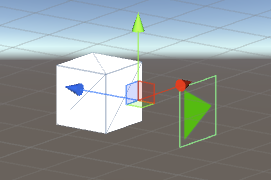
\includegraphics[width=0.3\textwidth]{images/action_prefab.png}
  \caption{Botones de acci�n formados por un cubo y un sprite con el
    fondo transparente.}
  \label{s5:fig:sction_prefab}
\end{figure}

Para poder interactuar con el bot�n, el sprite tiene asociado un
componente de colisi�n en 2D, permitiendo detectar cuando es
pulsado. Para cambiar el color del fondo, basta con buscar el �nico
\emph{MeshRenderer} del prefab (el �nico que existe es el asociado al
cubo).


Asociado al sprite del prefab, se encuentra el siguiente script
(\texttt{Action.cs}), que posee una definici�n de todos los tipos de
acciones, as� de las acciones a realizar cuando el bot�n es pulsado:

\begin{lstlisting}[caption={Action.cs Script encargado de reaccionar
      frente a las pulsaciones de los botones}]
using UnityEngine;
using System.Collections;

/**
 * Posibles tipos de comandos
 */
public enum ActionType{
	up,
	right,
	left,
	jump,
	play,
	light,
	trash,
	pause,
	p1,
	p2,
	none
}

/**
 * Listener de las pulsadciones de los botones. Segun el comando a ejecutar
 * invoca a un metodo u otro 
 */
public class Action : MonoBehaviour {
  //Tipo de accion que representa el boton
  public ActionType actionType;
  
  
  
  public void OnMouseUpAsButton()
  {
    switch (this.actionType) {
      case ActionType.play:
        Director.S.play();
        break;
      case ActionType.trash:
        Director.S.trash();
	break;
      case ActionType.none: //si pulsamos en una accion vacia, es que estamos en el panel
        Panel p = transform.parent.transform.parent.GetComponent<Panel>(); 
	p.activatePanel();
	break;
      default: //acciones para el robot
      Director.S.addAction (this.actionType);
      break;
    }
  }
}
\end{lstlisting}


\subsection{Layout}
\label{s5:subsec:layout}
Para la creaci�n de la interfaz derecha de la pantalla, partimos de la
configuraci�n inicial de la pantalla mostrada en la
figura~\ref{s5:fig:interfaz_white} (es decir, los
siguientes prefabs ya se encuentran instanciados en la escena, no a
trav�s del c�digo):

\begin{figure}[h]
  \centering
  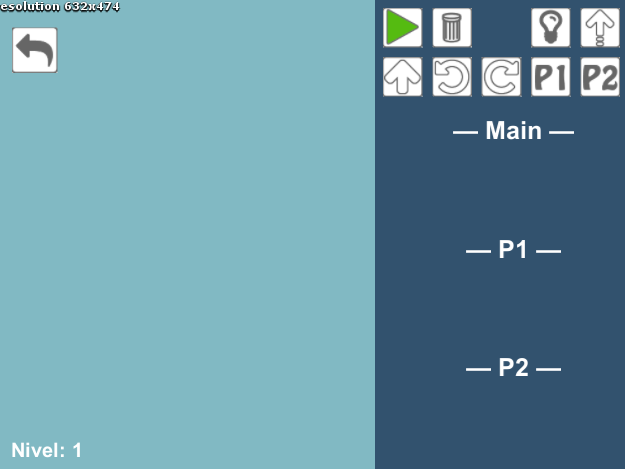
\includegraphics[width=0.6\textwidth]{images/interfaz_white.png}
  \caption{Prefabs instanciados en la escena.}
  \label{s5:fig:interfaz_white}
\end{figure}

Para crear el resto de la interfaz, se utiliza el script
\texttt{Action\_layout.cs}, que crea los paneles en los que insertar
las acciones, y sirve de medio entre el ``Director'' del juego y los
paneles (para colorearlos, cambiar el fondo, limpiarlos, ...). El
c�digo de este script es el siguiente:

\begin{lstlisting}[caption={Script encargado de la interfaz derecha.}]
using UnityEngine;
using System.Collections;
using System.Collections.Generic;

/**
 * Script que se encarga de la interfaz de la parte derecha.
 * Comandos, paneles y demas
 */
public class Actions_Layout : MonoBehaviour {
  public static Actions_Layout S; //Singleton para poder acceder
  
  public GameObject panelPrefab; //Prefab para construir los paneles de comandos

  // Esta pareja relaciona el sprite con el tipo de accion. Sirve para modificar los paneles de ordenes
  public List<Sprite> arrows_sprite; 
  public List<ActionType> actions_type; 
  
  //Sprites para el boton de play/stop
  public Sprite play_Sprite;
  public Sprite stop_Sprite;
  public bool playStatus; //Estamos reproduciendo o grabando ordenes?
  
  
  public bool _________________________;
  
  
  public float panelOffset = -3.0f; //ofset entre paneles para colocarlos
  
  public List<Panel> paneles; //lista de los paneles segun se van creando
   
  
  public void Awake(){
    S = this;
  }
  
  public void Start(){
    this.playStatus = true;
    this.createPanels(3); //en un principio solo creamos 3 paneles
    
    this.paneles[0].activatePanel(); //El primer panel es el activo
  }
  
  
  // Crea num paneles a partir del prefab y los posiciona segun el offset. 
  // Guarda los paneles en el atributo para poder acceder
  public void createPanels(int num){
    for (int i=0; i<num; i++) {
      GameObject go = Instantiate (this.panelPrefab);
      Panel p = go.GetComponent<Panel> ();
      
      p.buildPanel(12, i);
      p.transform.localPosition = new Vector3(p.transform.position.x,
      p.transform.position.y + i*this.panelOffset,
      p.transform.position.z);
      this.paneles.Add (p);
    }  
  }
  
  // Dada una accion pasada por parametro (at), la inserta en el
  // panel numero n
  public void insertInPanel(int n, ActionType at){
    if (n > this.paneles.Count) //puede que no haya paneles 
       return;
    

    //Buscamos la figura a dibujar
    int i = 0;
    for (i=0; i<this.actions_type.Count; i++)
      if (this.actions_type [i] == at)
        break;


    //Comprobacion por si las moscas
    if (i > this.arrows_sprite.Count)
      return;


    //insertamos en el panel
    this.paneles[n].insertCell(this.arrows_sprite[i]);
  }
  
  
  // Por cada panel, elimina los colores del fondo (estado activo)
  public void switchOffAllLights(){
    foreach(Panel p in this.paneles){
      p.switchOffAllLIghts();  
    }
  }

  // Dado el numero de panel, ilumina o apaga (status) la casilla numero i
  public void lightCube(int panel, int i, bool status){
    if (this.paneles.Count <= panel)
      return;

    this.paneles [panel].SwitchLight (i, status);
  }

  //Resetea todos los paneles
  public void clearPanels(){
    foreach (Panel p in this.paneles) {
      p.clear ();
    }
  }

  //Resetea toda la interfaz. Basta con resetear todos los paneles
  public void restartLayout(){
    foreach (Panel p in this.paneles){
      p.restartPanel();
    }
  }

  // Cambia el boton de play por el de stop y viceversa
  public void changeButton(){
    SpriteRenderer sprr = (SpriteRenderer)(GameObject.Find("Action_play").GetComponentInChildren<SpriteRenderer> ());

    sprr.sprite = (this.playStatus) ? this.stop_Sprite : this.play_Sprite;
    this.playStatus = ! this.playStatus;
  }
}
\end{lstlisting}


\subsection{Panel}
\label{s5:subsec:panel}

Los distintos paneles en los que insertar las acciones vienen dados
por un \emph{GameObject} vac�o, con un script asociado. Este script es
el que crea el panel entero de manera procedural, a partir de los
atributos puestos a trav�s de la interfaz de Unity. El script
encargado de realizar esta tarea es \texttt{Panel.cs}, y aparte de
crear los paneles, tambi�n posee m�todos para cambiar el color de
fondo, iluminar una o varias celdas, borrarlo y modificar un sprite
por otro.

\begin{lstlisting}[caption={Script encargado de crear y administrar
      los paneles de acciones}]
using System.Collections;
using System.Collections.Generic;


/** Esta clase representa un panel al que se le pueden incorporar las distintas
 * acciones a realizar. Se crea con el numero te celdas solicitadas.
 * Asimismo, tiene metodos para iluminar el elemento de alguna posicion. 
 * Este panel no guarda informacion de las acciones de cada casilla, solamente esta
 * para controlar la parte grafica */

public class Panel : MonoBehaviour {

  public int numColumns;//tama�o del panel
  
  public GameObject celdaPrefab;//Prefab para construir el panel
  
  public Sprite nullSprite;	//Sprite nulo
  
  
  public float leftCorner = -2.5f; //Coordenadas para saber donde empezar a colocar
  
  
  //materiales para cambiar el color de fondo
  public Material lightOff_mat;
  public Material lightOn_mat;
  
  
  public bool ______________________;
  
  
  public List<GameObject> celdas;
  
  // Id del panel.
  public int _id;
  
  //indica cuantas celdas validas hay para insertar la siguiente
  public int numRellenos;
  
  
  // Construye el panel con el tama�o y el id pasados. Utiliza el prefab como celdas nulas.
  public void buildPanel(int size, int id){
    this._id = id;

    GameObject go;
    for (int i=0; i < size; i++) {
      go = Instantiate (this.celdaPrefab);
      go.transform.parent = this.transform;
      
      go.transform.localPosition = new Vector3 (this.leftCorner + (i % this.numColumns), -1 * (i / this.numColumns), 0);
      
      this.celdas.Add (go);
    }
    
    this.numRellenos = 0;
  }
  
  
  //Elimina todas las celdas del panel y las vuelve a crear nulas
  public void restartPanel(){
    this.numRellenos = 0;
    int tam = this.celdas.Count;
    foreach (GameObject g in this.celdas)
       Destroy(g);

    this.celdas = new List<GameObject>();
    this.buildPanel(tam, this._id);
  }


  //Modifica la celda actual por el sprite pasado por parametro
  public void insertCell(Sprite spr){
    if (this.numRellenos >= this.celdas.Count)
      return;

      SpriteRenderer sprr = this.celdas [numRellenos++].GetComponentInChildren<SpriteRenderer> ();
      sprr.sprite = spr;
  }


  //Modifica el fondo de todas las celdas a apagado
  public void switchOffAllLIghts(){
    for(int i=0; i<this.celdas.Count; i++)
      this.SwitchLight(i, false);
  }

  //Modifica el fondo de una celda en concreto
  public void SwitchLight (int i, bool status){
    if (i >= this.celdas.Count)
      return;

      Material newmat = status ? this.lightOn_mat : this.lightOff_mat;

      MeshRenderer rmat;
      rmat = this.celdas[i].GetComponentInChildren<MeshRenderer>();
      rmat.material = newmat;				
      
  }
  
  // Modifica todas las celdas para ponerlas a null
  public void clear(){
    SpriteRenderer sr;
    
    for(int i=0; i<this.celdas.Count; i++){
      sr = this.celdas[i].GetComponentInChildren<SpriteRenderer>();	
      sr.sprite = this.nullSprite;
    }
    this.numRellenos = 0;
  }
  

  //Colorea todas las celdas del panel con el fondo activo
  public void activatePanel(){
    //coloreamos a todas las celdas para que esten activas
    for(int i = 0; i<this.celdas.Count; i++)
      this.SwitchLight(i, true);
    
    //avisamos al director
    Director.S.panelActive(this._id);
  }

  //Colorea todas las celdas del panel con el fondo desactivado
  public void deactivatePanel(){
    //borramos el color de todas las celdas
    for(int i = 0; i<this.celdas.Count; i++)
      this.SwitchLight(i, false);
  }
}
\end{lstlisting}

\newpage{}

\section{Coordinaci�n entre las dos interfaces: El director de orquesta}
\label{s6:sec:director}

Para la gesti�n entre las dos interfaces (la que graba las acciones del
usuario y el robot que las reproduce), se utiliza un script llamado
\texttt{Director.cs}. Este script realiza m�ltiples acciones, aunque las
m�s importantes son las siguientes:
\begin{itemize}
  \item Almacena las acciones que va introduciendo el usuario, y manda al
    panel correspondiente que la pinte.
  \item Gestiona el panel activo. Manda colorear al panel correspondiente.
  \item Reinicia la interfaz correspondiente cuando el jugador pulsa alg�n
    bot�n que desencadene esta acci�n (stop o basura).
  \item Reproduce los comandos en orden utilizando una estructura de pila.
\end{itemize}

\subsection{Reproduciendo los comandos}
A la hora de reproducir comandos se presentan dos retos que afrontar:
\begin{enumerate}
  \item Hay que mantener la traza de ejecuci�n para poder colorear el
    comando activo y eliminar el anterior.
  \item Tiene que ser v�lido para llamadas recursivas.
\end{enumerate}

Los comandos se encuentran almacenados en tres listas, una para cada
procedimiento (\emph{Main}, \emph{P1} y \emph{P2}). Para reproducirlos en
orden y almacenar la traza se utiliza una pila basada en ciclos. En cada
inicio de ciclo se desapila la acci�n a realizar junto con el panel del que
realizarlo, y al finalizar el ciclo, se apila la nueva acci�n junto con el
panel correspondiente. La gesti�n de esta pila, junto con el resto de
m�todos del script es la siguiente:\\

\begin{lstlisting}[caption={Director.cs}]
using UnityEngine;
using System.Collections;
using System.Collections.Generic;

/**
 * Estructura auxiliar usada para la reproduccion de los comandos
 */
struct PairInt {
  public PairInt(int a, int b) {
    x = a;
    y = b;
  }
  public int x, y;
}


/**
 * Director de orquesta. Es el encargado de llevar el control de todo el juego.
 * Maneja los paneles y controla las acciones pulsadas.
 * Almacena la lista de todas acciones a ejecutar.
 * La reproduccion la reliza mediante un sistema de pilas.
 * Avisa al layout para colorear/descolorear las celdas.
 * Controla la victoria del juego
 */
public class Director : MonoBehaviour {
  public static Director S; //Singleton
  
  public int totalGoals; //Numero de objetivos. Usado para condicion de victoria
  public GameObject texto; //Texto a mostrar cuando se supera un nivel
  
  public bool ______________________________;
  
  public List< List<ActionType> > acciones; //Lista de lista de acciones. Por cada panel existe una lista de acciones.
  public bool recording; //Bool indicando si se esta reproduciendo o grabando acciones
  public int panelActiveId; // Int indicando el panel actual activo
  
  
  private Stack<PairInt> llamadas; //Pila utilizada para realizar la reproduccion de los comandos
  
  
  
  public void Awake(){
    S = this;
  }
  
  
  public void Start(){
    this.recording = true;
    
    this.acciones = new List<List<ActionType>> ();
    this.acciones.Add(new List<ActionType>());
    this.acciones.Add(new List<ActionType>());
    this.acciones.Add(new List<ActionType>());
  }
  
  
  // A�ade la accion pasada por parametro al panel actual.
  // Guarda la accion en la lista de acciones local.
  public void addAction(ActionType at){
    if (!this.recording)
      return;

    this.acciones[this.panelActiveId].Add (at);
    Actions_Layout.S.insertInPanel (this.panelActiveId, at);
  }


  // Ejecuta los comandos que estaban guardados
  // Para ello, apila en una pila parejas <int,int>, que representan 
  // <panelId, ActionId>. Simula una pila de llamadas de funciones.
  public void play(){
    Actions_Layout.S.changeButton();
    
    if (this.recording) {
      this.recording = false;
      this.llamadas = new Stack<PairInt>();
      this.llamadas.Push(new PairInt(0,0));
      Actions_Layout.S.switchOffAllLights();
      
      Next ();
    }else{
      this.restartLevel();
    }
  }
  
  
  // Ejecuta la siguiente accion.
  // Utiliza el sistema de pila para simular las llamadas a funcion.
  // De esta maenra se consiguen llamadas recursivas, y coloreado de la
  // interfaz.
  public void Next(){
    if (this.recording)
      return;
    
    if (this.llamadas.Count > 0) {
      PairInt pi = this.llamadas.Pop ();
      
      if(pi.y < 0){ //si acabamos una rutina, apagamos el ultimo elemento
	Actions_Layout.S.lightCube (pi.x, this.acciones[pi.x].Count-1, false);
	Invoke("Next", 1);
      }else
        this.ejecutaAccion (pi.x, pi.y);
    }
  }
  
  
  //Ejecuta la accion i sobre la lista a, y apila la siguiente en la pila de llamadas
  public void ejecutaAccion(int a, int i){
    
    //apagamos la anterior si podemos
    if (i > 0)
      Actions_Layout.S.lightCube (a, i - 1, false);
    //enciende la actual
    Actions_Layout.S.lightCube (a, i, true);
    
    //apilamos la sigiente ejecucion, si existe
    if (i + 1 < this.acciones [a].Count)
      this.llamadas.Push (new PairInt (a, i + 1));
    else
      this.llamadas.Push (new PairInt (a, -1));


    switch (this.acciones[a][i]) {
      case ActionType.up:
        Robot.S.moveUP ();
	break;
      case ActionType.jump:
        Robot.S.jump();
	break;
      case ActionType.right:
        Robot.S.rotateRight();
	break;
      case ActionType.left:
        Robot.S.rotateLeft();
        break;
      case ActionType.light:
        int ret = GUI_Layout.S.SwitchLight(Robot.S.x,Robot.S.z);
	if (ret > 0) this.totalGoals --; 
	if (ret < 0) this.totalGoals++;

	testGoal();
	Invoke("Next",1);
	break;
      case ActionType.p1:
        this.llamadas.Push(new PairInt(1, 0));
	Invoke("Next", 1);
	break;
      case ActionType.p2:
        this.llamadas.Push (new PairInt(2,0));
  	Invoke("Next", 1);
	break;
      default:
      break;
    }
  }
  

  // Comprueba si se ha alcanzado la condicion de victoria
  public void testGoal(){
    if (this.totalGoals == 0) {
      this.recording = true;
      this.texto.SetActive(true);
      
      levelLoad.levelPassed[levelLoad.level-1] = true;
      Invoke("LoadMenu", 2);
    }
  }
  
  public void LoadMenu(){
    Application.LoadLevel("_Scene_menu");
  }
  
  
  // Es llamado cuando se desea borrar todas las acciones.
  // Vacia la lista local y manda la orden a la interfaz
  public void trash(){
    if (!this.recording)
      return;
      
    for(int i=0; i<this.acciones.Count; i++)
      this.acciones[i].Clear ();
        
      Actions_Layout.S.clearPanels ();
  }

  
  public void restartLevel(){
    this.recording = true;
    
    GUI_Layout.S.restartLayout();
    Actions_Layout.S.switchOffAllLights();
    
    this.panelActiveId = 0;
    Actions_Layout.S.paneles [0].activatePanel ();
  }
  
  
  // Almacena el panel activo y ordena que se pinte al nuevo.
  // Apaga el panel activo viejo
  public void panelActive(int i){
    if(i != this.panelActiveId)
      Actions_Layout.S.paneles[this.panelActiveId].deactivatePanel();
      
      this.panelActiveId = i;     
  }
}
\end{lstlisting}

\newpage{}

\section{El men� del juego}
El men� del juego viene representado en la figura~\ref{s7:fig:menu}. Los
botones est�n creados de igual manera que las acciones vistas en las
secciones anteriores. Asociado a cada bot�n hay un script encargado de
cargar el men� correspondiente y colorear el fondo de acuerdo a si se ha
superado o no. Para realizar la carga de niveles y almacenar los niveles
superados se utiliza una clase est�tica.
\begin{figure}
  \centering
  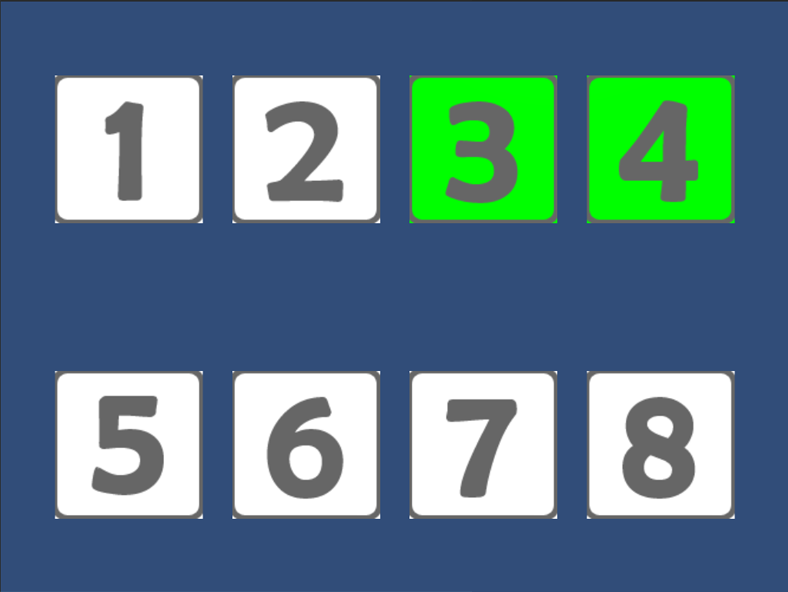
\includegraphics[width=0.7\textwidth]{images/interfaz_menu.png}
  \caption{Escena con el men�}
  \label{s7:fig:menu}
\end{figure}


\begin{lstlisting}[caption={Menu.cs}]
using UnityEngine;
using System.Collections;

/**
 * Clase estatica que almacena el estado actual de los niveles, asi como del nivel actual
 **/
public static class levelLoad{
  public static int level = -1;
  public static bool[] levelPassed = {false, false, false, false,
    false, false, false, false};
}


/**
 * Listener de los botones del menu. Carga el menu correspondiente
 **/
public class Menu : MonoBehaviour {

  public int level;
  public Material bck_green;
  

  //Comprobamos si el nivel se ha superado y lo pintamos de verde
  public void Start(){
    //cambiar el material del fondo
    if(levelLoad.levelPassed[this.level-1]){
      MeshRenderer rmat;
      rmat = this.transform.parent.GetComponentInChildren<MeshRenderer>();
      
      rmat.material = this.bck_green;	
    }
  }
  

  public void OnMouseUpAsButton(){
    if(this.level==0){ //cargamos el menu
      Application.LoadLevel("_Scene_menu");
    }
    else {//caso contrario cargamos el nivel correspondiente
      levelLoad.level = this.level;
      
      Application.LoadLevel("_Scene_0");
    }
  }
}
\end{lstlisting}

\newpage{}

\section{Caracter�sticas principales de la implementaci�n}
Las caracter�sticas principales de la implementaci�n del juego vienen
resumidas a continuaci�n:

\begin{itemize}
\item Se utilizan dos c�maras para componer la interfaz del juego. Cada
  c�mara muestra subespacio de la escena. La interfaz de cada c�mara se
  encuentra gestionada por su propio script.
\item Dise�o de niveles a trav�s de una estructura xml. Permite crear y
  modificar niveles de manera sencilla.
\item Utilizaci�n de sprites para la creaci�n de botones.
\item utilizaci�n de distintos materiales desde el c�digo que permite
  cambiar el fondo de los botones y algunos aspectos.
\item Utilizaci�n de curvas de Bezier para el movimiento de salto del
  robot, produciendo un movimiento m�s natural. Los movimientos se
  implementan en un componente aparte permitiendo su reutilizaci�n,
  mientras que la l�gica de los movimientos (saber si se puede mover o no),
  la implementa el componente Robot.
\item Control de errores antes de ejecutar una acci�n. Si el robot no es
  capaz de ejecutar una acci�n, contin�a ejecutando la siguiente.
\item Creaci�n de un sistema basado en una pila para simular la
  reproducci�n de los comandos. Permite generar una traza de la ejecuci�n
  (mostrada en formato visual mediante los colores del fondo de las
  acciones), y simular llamadas recursivas y llamadas anidadas.
\item Utilizaci�n de dos escenas: la escena de men� y la escena de juego.
\item La escena de juego es la misma para todos los niveles, lo que se
  cambia es el fichero xml desde el que leer el mapa.
\item Para la gesti�n entre el men� y la escena del juego, as� como para
  almacenar los niveles superados se utiliza una clase est�tica que
  permanece instanciada durante toda la ejecuci�n.
\item La creaci�n de los paneles donde insertar los comandos se realiza de
  forma procedural, permitiendo crear tantos paneles como sean necesarios,
  as� como elegir el tama�o de cada uno de los paneles.
\end{itemize}



\newpage{}
\bibliographystyle{plain}
\bibliography{references} 


\end{document}



%
%
%%%
%%% Local Variables:
%%% mode: latex
%%% TeX-master: "./main.tex"
%%% End:

